\chapter{Initial Data Analysis}\label{Sec:Initial Data Analysis}

In order to diagnose to what extent an algorithm suffers from sampling bias, it will be useful to have another dataset. Initial data analysis is conducted independently of the problem statements to understand what properties of the data differ between GBS and GESIS for matching attributes. A brief characterization of the data currently employed in the studies is given in this chapter. The GitHub repository further specifies the list of transformations that are sequentially applied to each group of features in order to prepare the inputs for survey comparisons. Preprocessing steps and methods used to evaluate outcomes are documented as well. Scaling methods that apply to both data sets, e.g: centering and scaling of skewed continuous features for SVMs, are not mentioned but can be deduced from code easily. If an attribute is removed at some point, it will only be mentioned in the relevant section.

\begin{figure}[ht]
	\begin{center}
		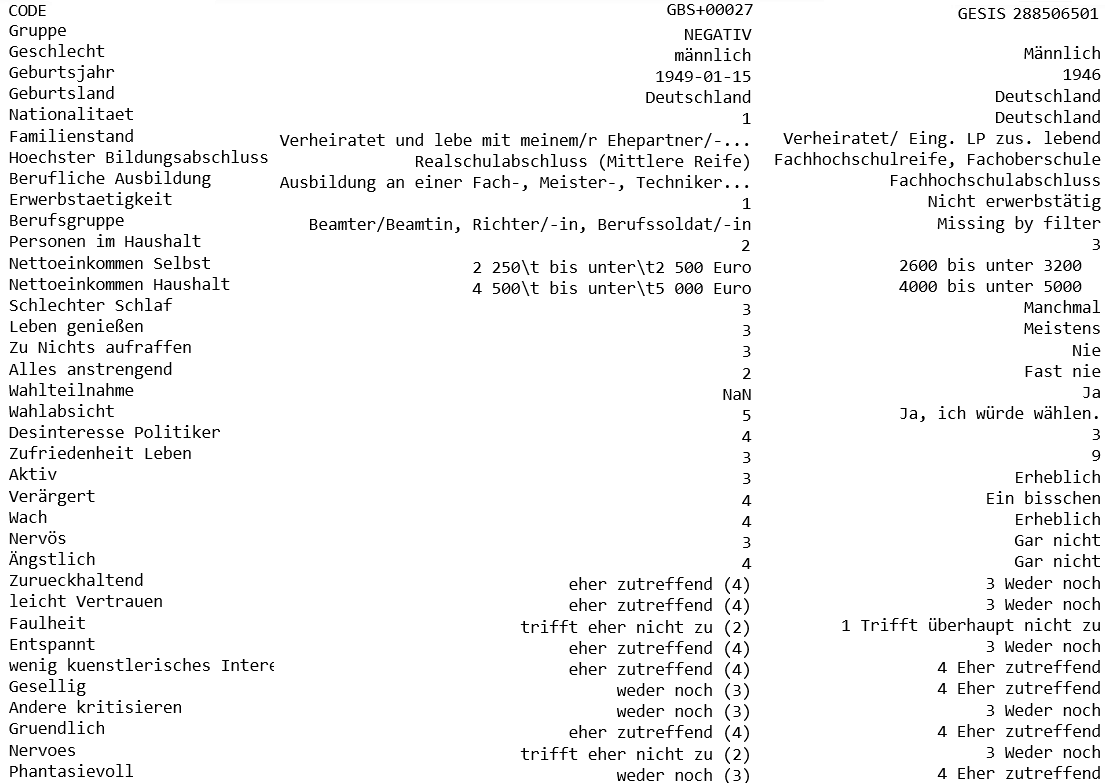
\includegraphics[scale=0.52,angle=0]{fig/values_compare}
		\label{std}
		\caption{GBS - GESIS attribute and value comparison. Not all attributes are used in every learning task. See GitHub documentation for more information.}
	\end{center}
\end{figure}

\section{Feature Selection and Data Imputation}

Missing values in GESIS and GBS need to be handled first to clarify preprocessing steps and simplify future work on political participation and resilience. Note that the figure represents the data after attribute and value matching and before potential data imputation. This graphic also lends itself to first thoughts about whether missing data elements depend on observable and unobservable attributes or occur entirely at random and is also able to detect functional dependencies in survey data. Figure X summarizes the main observations from GESIS, figure Y summarizes the main obersvations in GBS. The correlation matrix (Fig Z) with ratio -1 to +1 is used as another way to visualize differences in GESIS and GBS and to further simplify preprocessing decisions. Potential bugs and issues can also be detected with this graph. 

If not stated differently, deletion of rows is applied to every instance with missing values in GESIS to reduce the class imbalance in the later described classification problem. Missing values are sparse in GBS and can be imputed, e.g: with median substitution, with negligible effects. Mean substitution can not be used as this might lead to new unseen values. 

\section{Likert-Type Scale}

\subsection{The Big Five Dimensions}

The Big Five is an empirically-derived model of human personality and psyche. When factor analysis is applied to personality survey data, five clusters of traits consistently emerge. The BFI-10 is a 10-item scale measuring the Big Five personality traits, two BFI items for each dimension, representing both the high and low pole of each factor [Fig X]. Likert scales are the most frequently used instruments in GBS and GESIS. They consist of statements which measure the intensity of one's estimation towards the preceding statement. Respondents are asked to rate the BFI-10 items on a level of agreement on a consistent rating scale ranging from "Strongly Agree (5)" to Strongly Disagree (1)" for all items in both survey.

\begin{figure}[H]
	\begin{center}
		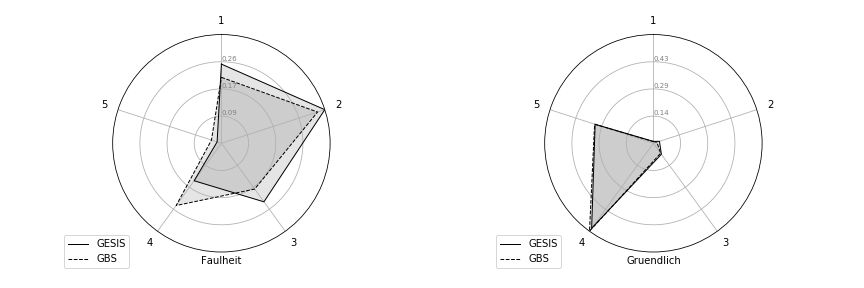
\includegraphics[scale=0.52,angle=0]{fig/Conscientiousness_figure}
		\label{Conscientiousness}
		\caption{Conscientiousness is the degree of organization, self-regulation, and responsibility one exhibits. \textit{"I see myself as someone who tends to be lazy."}(left). \textit{"I see myself as someone who does a thorough job."}(right).}
	\end{center}
\end{figure}

 is still ongoing debate on whether to use a Likert scale item as categorical or numeric feature. The intervals between positions on the scale are monotonic but never so well-defined as to be numerically uniform increments. A "Strongly Agree (5)" response indicates more agreement than "Agree", but it does not show agreement that is five times stronger than "Strongly Disagree (1)". 

There is an underlying measurement continuum, but  
This project treats the responses as if they fell on an interval scale.

Figure X. shows the response distribution of values for "Conscientiousness" of GBS and GESIS participants (see Appendix for a visualization of distribution shifts in "Agreeableness", "Openness", "Extraversion" and "Neuroticism").

Since GESIS and GBS analyse  on a group level should be relatively insensitive to problems that may arise.

In all these cases each aggregate measure (perhaps the mean) is based on many individual responses (e.g., n=50, 100, 1000, etc.). In these cases the original Likert item begins to take on properties that resemble an interval scale at the aggregate level.
life satisfaction of states or countries,
job satisfaction of departments,

The graphs are almost identical for the Likert item "Gruendlich". 

The cyclic structure of the chart, i.e. "Strongly Disagree" next to Strongly Agree", provides a vivid example for the central-tendency bias across all items.

\subsection{Data Mismatch}

\begin{table}[ht]
    \begin{center}
            {\footnotesize
            \begin{tabular}{l|c|ccccccccc}
                \hline \hline
		Raw Data & GESIS & 1 & 2 & 3 & 4 & 5 & 6 \\
                     & GBS & 1 & 2 & 3 & 4 & 5 & \\
                \hline
		Max Scaler & GESIS & 0.83 & 1.7 & 2.5 & 3.3 & 4.2 & 5.0 \\
                     & GBS & 1 & 2 & 3 & 4 & 5 & \\
                \hline
		Min-Max Scaler & GESIS & 1 & 1.8 & 2.6 & 3.4 & 4.2 & 5 \\
                     & GBS & 1.0 & 2.25 & 3.5 & 4.75 & 6.0 & \\
                \hline
		Cut-Off Mapping & GESIS & 1 & 2 & 3 & 4 & 5 & 5 \\
                     & GBS & 1 & 2 & 3 & 4 & 5 & \\
\hline \hline
            \end{tabular}}
        \caption{Different value scalings of attribute "Desinteresse Politiker".}
\label{Tab:DescripStatsRawData}
\end{center}
\end{table}

Shortcomings in attribute mappings may result in inappropriate representation and incorrect conclusions.

\begin{table}[ht]
    \begin{center}
            {\footnotesize
            \begin{tabular}{l|c|ccccccccc}
                \hline \hline
		attribute & GBS values & GBS values count &  GBS values & GBS values count \\
                \hline \hline
                     Wach & 4 & 311 & Einigermassen & 1697 \\
                     & 3 & 183 & Erheblich & 1389 \\
                     & 2 & 66 & Ein bisschen & 467 \\ 
              	& 1 & 14 & Aeusserst & 367 \\	
		& -1 & 1 & Gar nicht & 184 \\		
		& -9 & 1 & & \\
	     \hline \hline
            \end{tabular}}
        \caption{Caption.}
\end{center}
\end{table}


\begin{figure}[ht]
	\begin{center}
		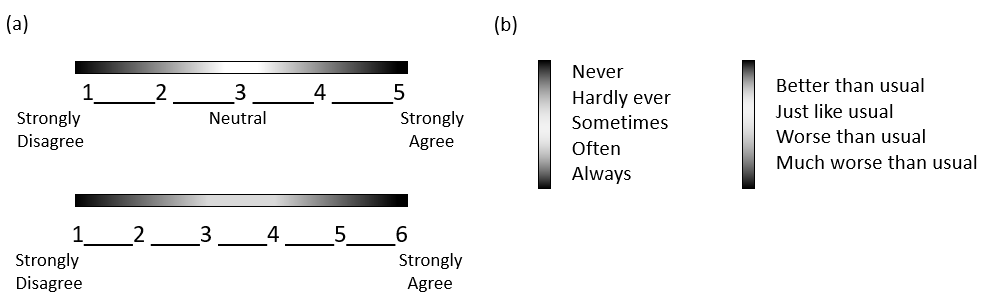
\includegraphics[scale=0.50,angle=0]{fig/scales}
		\label{6_5}
		\caption{Example of a Likert item discrepancy. GBS uses an odd number of responses with a "neutral" option, such as "no opinion", "neither agree nor disagree" or some phrase to that effect. In contrast, there is an even number of responses for this item in GESIS encouraging participants to voice a positive or negative opinion.}
	\end{center}
\end{figure}


\begin{figure}[ht]
	\begin{center}
		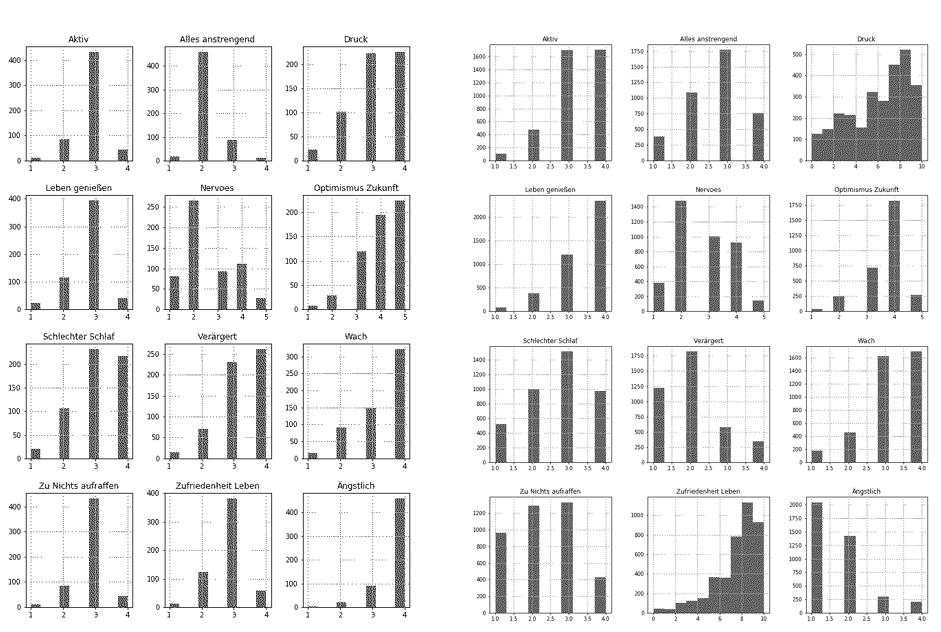
\includegraphics[scale=0.62,angle=0]{fig/histo}
		\label{std}
		\caption{GESIS hists.}
	\end{center}
\end{figure}

Inconsistencies are discovered later with the planned learning models as 

John Tukey wrote otherwise (back in 1960) in a monograph "Data Analysis and Behavioral Science" (published in Collected Works v. III). One result he obtained is that if you're getting better than about 10percent test-retest agreement, your scale isn't narrow enough!

[1] It is confirmed that different numbers of rating bars in a subjective rating scale can have significant effects on the subjective measurement, thus the assessment of the Big Five dimensions of personality.

Techniques for reducing the length of scales while maintaining psychometric quality.
Figure X shows an example of such as a statement.

In some cases, an additional "opt-out" option is provided for those respondents who truly cannot respond in GBS only.

